\chapter{Studi Literatur}

\section{Pembelajaran dan Pemrograman}
\subsection{Pembelajaran}
Menurut \textcite{slavin2017learn}, belajar adalah perubahan yang relatif permanen dalam perilaku atau potensi perilaku sebagai hasil dari pengalaman atau latihan yang diperkuat. Belajar merupakan akibat adanya interaksi antara stimulus dan respons. Seseorang dianggap telah belajar sesuatu jika dia dapat menunjukkan perubahan perilakunya. Menurut teori ini, dalam belajar yang penting adalah input yang berupa stimulus dan output yang berupa respons.

Teori lain mengenai pembelajaran juga dikemukakan oleh \textcite{gagne1970learning} bahwa pembelajaran adalah seperangkat peristiwa-peristiwa eksternal yang dirancang untuk mendukung beberapa proses belajar yang bersifat internal. Pembelajaran terdiri dari beberapa tipe dan setiap tipe membutuhkan instruksi yang berbeda-beda. Menurut \textcite{gagne1970learning}, terdapat 5 kategori utama dalam pembelajaran: informasi verbal, kemampuan intelektual, strategi kognitif, kemampuan motorik, serta sikap. Setiap kategori memiliki kondisi internal dan eksternal masing-masing dalam proses pembelajarannya.

Menurut \textcite{gagne1985learning}, terdapat 9 peristiwa instruksi, yaitu: Perhatian dan Motivasi, Pemberitahuan Objektif Pembelajaran, Stimulasi Pengulangan, Pemberian Tantangan (Stimulus), Memberikan Arahan, Keterlibatan Langsung/Pengalaman, Memberikan Saran, Penilaian Performa, serta Meningkatkan Daya Ingatan. Dengan memanfaatkan peristiwa-peristiwa instruksi tersebut, instruktor dapat mempercepat pembelajaran internal pelajar. Hal-hal ini dapat dipakai dalam teknik pembelajaran sehingga hasil pembelajaran menjadi lebih efektif dan bertahan lama.

\subsection{Pemrograman}
Pada masa awal publikasi dalam pemrograman, banyak praktisi yang menjelaskan pemrograman sebagai proses yang menerjemahkan bahasa yang diketahui manusia menjadi bahasa yang dimengerti oleh mesin \parencite{mccracken1957digital}. \textcite{booth1958programming} menambahkan hubungan antara pemrograman dengan kalkulasi bahwa "Proses mengorganisasi kalkulasi dapat dibagi menjadi dua bagian -- fondasi formula matematis dan pemrograman yang sebenarnya ... menerjemahkan ... ke dalam bahasa mesin komputasi". \textcite{hartree2012calculating} menjelaskan bahwa "Proses mempersiapkan kalkulasi untuk mesin dapat dibagi menjadi 2 bagian, 'pemrograman' dan 'pengkodean'. Pemrograman adalah proses menggambarkan penjadwalan dari urutan operasi-operasi individu yang dibutuhkan untuk melakukan kalkulasi" \parencite{hartree2012calculating}.

Definisi pemrograman berubah seiring waktu dari domain matematika menjadi domain pemrosesan data yang lebih umum \parencite{hoc1990psychology}. Pada awalnya, pemrogram adalah orang yang serius dalam dunia komputer. Namun seiring dengan waktu, aplikasi-aplikasi besar banyak yang mulai menerapkan pemrograman untuk \textit{scripting} atau \textit{macro} sehingga definisi pemrograman dapat meluas hingga ke \textit{end-user} \parencite{goodell1999enduser}. Hal ini membuat \textcite{blackwell2002programming} mengusulkan bahwa pemrogram bisa menjadi siapapun yang menggunakan komputer dengan penggunaan yang berbeda-beda tergantung pada kegunaan dan kebutuhan.

\subsection{Pembelajaran Pemrograman}
Pembelajaran pemrograman merupakan aktivitas mempelajari pemrograman baik secara teori maupun praktik. Pembelajaran pemrograman merupakan kemampuan yang membutuhkan latihan praktis yang banyak \parencite{thomas2000student}. Hal ini membuat aktivitas praktik implementasi menjadi hal yang penting dalam proses pembelajarannya. Dalam pembelajaran tradisional, hal ini dapat dilakukan dengan adanya praktikum sehingga praktik implementasi dapat diarahkan oleh pengajar \parencite{choy2004interactive}. Selain itu, terdapat juga tugas-tugas berupa proyek mengimplementasikan program sesuai dengan spesifikasi yang dapat melatih pemecahan masalah pelajar.

Terdapat berbagai macam permasalahan yang sering terjadi pada orang yang baru mempelajari pemrograman. Menurut \textcite{moons2013pilot}, pengenalan pembelajaran pemrograman sering dianggap susah oleh pelajar sehingga menimbulkan retensi yang rendah. Permasalahan ini disebabkan oleh banyaknya konsep fundamental dan abstrak baru yang harus dipelajari dari pemrograman itu sendiri, sehingga diperlukan kemampuan kognitif yang kompleks untuk dapat memahami konsep-konsep tersebut. Selain itu, kurangnya kemampuan dalam menelusuri alur eksekusi program menjadi salah satu faktor dari permasalahan. \textcite{mayer1981psychology} menambahkan bahwa permasalahan ini juga disebabkan oleh belum terbentuknya model kerangka pikir terhadap cara program komputer bekerja sehingga pelajar baru dalam dunia pemrograman akan kesusahan dalam menerima informasi teknis yang baru selama proses pembelajaran pemrograman.


% Kayaknya yang bawah ini masuknya ke bab 3 aja
% Agar pelajar dapat benar-benar memahami (bukan hanya menghapal saja) konsep-konsep pemrograman baru, pelajar harus diberikan model konkret terlebih dahulu sebelum pemberian materi pemrograman sehingga dapat meningkatkan transfer pengetahuan dan pada akhirnya meningkatkan pemahaman konseptual.
% Sambungin juga ke solusi2 yang dipropose sama moon

\section{Pembelajaran Pemrograman secara Daring}
\subsection{Perkembangan Pembelajaran secara Daring}
Pembelajaran secara daring biasa digunakan untuk merujuk kepada pembelajaran berbasis web, pembelajaran terdistribusi, pembelajaran berbasis internet, pembelajaran siber, atau pembelajaran virtual \parencite{urdan2000elearning}. Pembelajaran secara daring adalah bagian dari pembelajaran jarak jauh yang memeluk berbagai macam aplikasi teknologi dan proses pembelajaran, termasuk pembelajaran berbasis komputer, pembelajaran berbasis web, kelas virtual, dan kolaborasi digital \parencite{urdan2000elearning}. Hal ini menunjukkan bahwa pembelajaran secara daring memiliki banyak sekali media yang dapat digunakan, mulai dari internet, siaran satelit, rekaman audio/video, CD, dll.

Pembelajaran secara daring bukanlah hal yang baru, namun dengan perkembangan teknologi zaman ini media pembelajaran secara daring semakin bervariasi dan kompleks. Penjelasan terkait perkembangan dalam pembelajaran secara daring dalam 30 tahun terakhir dapat dilihat pada \autoref{tab:sejarah-pembelajaran-daring} \parencite{keengwe2010towards}.

\small
\begin{longtable}{ |>{\setlength{\baselineskip}{0.75\baselineskip}}p{0.15\linewidth}|>{\setlength{\baselineskip}{0.75\baselineskip}}p{0.3\linewidth}|>{\setlength{\baselineskip}{0.75\baselineskip}}p{0.45\linewidth}| }
  \caption{Sejarah Perkembangan Pembelajaran secara Daring}\label{tab:sejarah-pembelajaran-daring}                                                                                                                                                                                                                                                              \\ \hline
  \rowcolor{gray!30}
  \textbf{Tahun} & \textbf{Fokus}                                                       & \textbf{Karakteristik Sistem Edukasi}                                                                                                                                                                                                                                 \\ \hline
  \endfirsthead
  %
  \caption*{\autoref{tab:sejarah-pembelajaran-daring} (lanjutan): Sejarah Perkembangan Pembelajaran secara Daring}                                                                                                                                                                                                                                              \\ \hline
  \rowcolor{gray!30}
  \textbf{Tahun} & \textbf{Fokus}                                                       & \textbf{Karakteristik Sistem Edukasi}                                                                                                                                                                                                                                 \\ \hline
  \endhead
  %
  1975-1985      & Pemrograman; Latihan Soal; \textit{Computer-assisted learning (CAL)} & Pendekatan pembelajaran secara behavioristik; Pemrograman untuk membangun alat dan pemecahan masalah; Interaksi pengguna-komputer secara lokal.                                                                                                                       \\
  \hline
  1983-1990      & Pelatihan multimedia berbasis komputer                               & Penggunaan model CAL terdahulu dengan integrasi multimedia interaktif; Dominansi model pelajar pasif; Influensi dari pembelajaran menggunakan alat peraga mulai terlihat.                                                                                             \\
  \hline
  1990-1995      & Pelatihan dan edukasi berbasis web                                   & Penyampaian materi melalui internet; Pengembangan model pelajar aktif; Pembelajaran dengan alat peraga menjadi umum; Interaksi pengguna secara terbatas.                                                                                                              \\
  \hline
  1995-2005      & \textit{E-learning}                                                  & Penyampaian materi melalui internet dengan lebih fleksibel; Peningkatan interaktivitas; Penggunaan kelas multimedia secara daring; Interaksi pengguna jarak jauh.                                                                                                     \\
  \hline
  2005- sekarang & Pembelajaran melalui gawai dan jaringan sosial                       & Adanya materi pembelajaran interaktif melalui \textit{Learning Management System} (LMS) dengan komponen jaringan sosial; Pembelajaran yang difasilitasi gawai nirkabel seperti ponsel dan laptop; Pembelajaran secara portabel dengan fokus kepada mobilitas pelajar. \\
  \hline
\end{longtable}
\normalsize

\subsection{Pembelajaran Interaktif dan \textit{Interactive Learning Environment} (ILE)}

Pada dasarnya, pembelajaran interaktif atau \textit{interactive learning} adalah pembelajaran yang melibatkan adanya interaksi antara pelajar dengan konten pembelajaran, baik itu dalam memproses materi, menyelesaikan tugas, atau memecahkan masalah dengan tujuan membangun kognitif, afektif, konatif, dan psikomotorik hasil dari pembelajaran \parencite{reeves2012interactive}. Secara singkatnya, terdapat hubungan aksi timbal-balik antara pelajar dan pengajar sehingga pembelajaran tidak menjadi pasif. Dalam konteks pembelajaran secara daring, hal ini dapat diwujudkan dengan adanya teknologi digital yang menghubungkan antara pelajar dan pengajar.

Ciri-ciri dari pembelajaran interaktif menurut \textcite{reeves2012interactive} adalah adanya akses menuju konten, tugas, dan persoalan oleh pelajar menggunakan teknologi digital seperti komputer yang memiliki akses internet. Lebih lanjut lagi, \textcite{reeves2012interactive} menjelaskan terdapat 2 pendekatan dalam pengaplikasian pembelajaran interaktif, yaitu pembelajaran "melalui" program pembelajaran interaktif dan pembelajaran "dengan" program pembelajaran interaktif. Pembelajaran "melalui" program pembelajaran interaktif artinya program memberikan materi yang dibalut dengan metode komunikasi yang beragam (berfokus pada penyampaian materi yang interaktif), sementara pembelajaran "dengan" program pembelajaran interaktif menggunakan kakas-kakas kognitif yang dapat digunakan oleh pelajar untuk membangun bagian-bagian informasi menjadi pengetahuan sehingga pelajar dapat membangun model representasi pemahamannya sendiri yang lebih familier. Pembelajaran "dengan" program pembelajaran interaktif jauh lebih berdampak karena dapat memfasilitasi pemikiran kritis dan \textit{higher order thinking} (HOT). Program atau lingkungan yang digunakan dalam pembelajaran interaktif ini disebut juga sebagai \textit{interactive learning environment} (ILE).

% Interaksi pelajar dengan pengajar dapat dengan mudah digambarkan pada pembelajaran tradisional. Karena dapat bertemu secara langung di tempat dan waktu yang sama, hal ini memungkinkan sejumlah interaksi atau hubungan timbal-balik antara pelajar dan pengajar, seperti melemparkan pertanyaan kepada siswa, meminta siswa memecahkan persoalan di depan kelas, dll. Namun, tidak semua hal tersebut dapat diadaptasi dalam pembelajaran secara daring karena tempat dan waktu antara pelajar dan pengajar dapat berbeda (asinkron). Di lain sisi, pembelajaran secara daring dapat membuka potensi baru dalam metode pembelajaran karena adanya integrasi dengan teknologi digital. Hal ini menimbulkan adanya lingkungan pembelajaran baru yang mendukung pembelajaran secara daring, yaitu lingkungan pembelajaran interaktif atau disebut juga sebagai \textit{interactive learning environment} (ILE).

ILE adalah sistem yang menggunakan perangkat lunak dan terkadang juga hingga perangkat keras khusus yang dapat mendukung pembelajaran dalam pendidikan \parencite{psotka2012ile}. Dengan adanya integrasi dengan internet dan berbagai macam perangkat, ILE memiliki banyak potensi bahkan dapat melebihi kemampuan dari pembelajaran tradisional karena terhubung dengan internet dan pesatnya peningkatan interaktivitas antara manusia dan komputer.

\subsection{Pembelajaran Pemrograman Interaktif}
\subsubsection{ILE dalam Pembelajaran Pemrograman}
Menurut \textcite{choy2004interactive}, dibutuhkan 4 komponen sistem agar dapat mendukung pembelajaran pemrograman secara daring, yaitu lingkungan yang mendukung aktivitas pemrograman secara praktis, interaksi pelajar dan pengajar secara asinkron, analisis dari hasil pekerjaan pelajar, serta manajemen distribusi dan pengumpulan tugas. Komponen yang mendukung aktivitas pemrograman secara praktis dimaksudkan untuk mempermudah pelajar melakukan aktivitas pemrograman di mana saja dan kapan saja. Karena sistem juga menyimpan progres pembelajaran, pelajar dapat melakukan pembelajaran pemrograman secara nyaman karena dapat melakukan aktivitas tersebut di perangkat manapun. Aktivitas mencakup penulisan kode, eksekusi kode, hingga pengetesan kode.

Terdapat beragam jenis bentuk lingkungan pembelajaran interaktif yang dapat mendukung pembelajaran pemrograman menurut \textcite{moons2013pilot}, seperti \textit{microworlds} yang menggunakan grafis seperti kura-kura LOGO ataupun dalam bentuk fisik robotik seperti Lego Mindstorm Kit yang menggunakan bahasa pemrograman sederhana, kakas visualisasi algoritma untuk memvisualisasikan alur kerja suatu algoritma spesifik, serta kakas visualisasi eksekusi program yang dapat menampilkan alur proses kerja suatu program saat dieksekusi. Situs-situs yang menawarkan pembelajaran secara daring, seperti \textcite{sololearn2021media}, \textcite{codesaya2021media}, \textcite{brilliant2021media}, serta portal pembelajaran lembaga pendidikan atau \textit{e-learning system} juga termasuk sebagai ILE dengan bentuk pendekatan pembelajaran interaktif pertama yang "melalui" pembelajaran interaktif karena bersifat statik.

Salah satu bentuk ILE yang digunakan dalam pembelajaran pemrograman adalah \textit{integrated development environment} (IDE) berbasis web (berikut disebut sebagai Web IDE), yang memungkinkan pelajar pemrograman dapat menuangkan kode serta menjalakannya. Hal ini dikarenakan Web IDE memungkinkan penggunanya untuk langsung mengimplementasikan kode tanpa harus melakukan penyetelan apapun terlebih dahulu. Web IDE juga dapat memastikan bahwa lingkungan eksekusi program akan selalu sama antara satu pengguna dengan pengguna lain, serta meningkatkan portabilitas karena bisa dikerjakan kapan dan di mana saja \parencite{tran2013interactive}. ILE ini dapat diintegrasikan dengan kakas visualisasi eksekusi program sehingga dapat meningkatkan pemahaman pelajar terhadap konsep-konsep pemrograman \parencite{moons2013pilot}. ILE seperti ini termasuk dalam pendekatan pembelajaran interaktif kedua yaitu "dengan" pembelajaran interaktif karena memberikan kakas yang dapat digunakan oleh pengguna untuk dieksplorasi lebih lanjut. Berikut adalah contoh ILE berupa visualisasi eksekusi kode yang dapat dilihat pada \autoref{fig:pythontutor} dan \autoref{fig:evizor}

\begin{figure}[H]
  \centering
  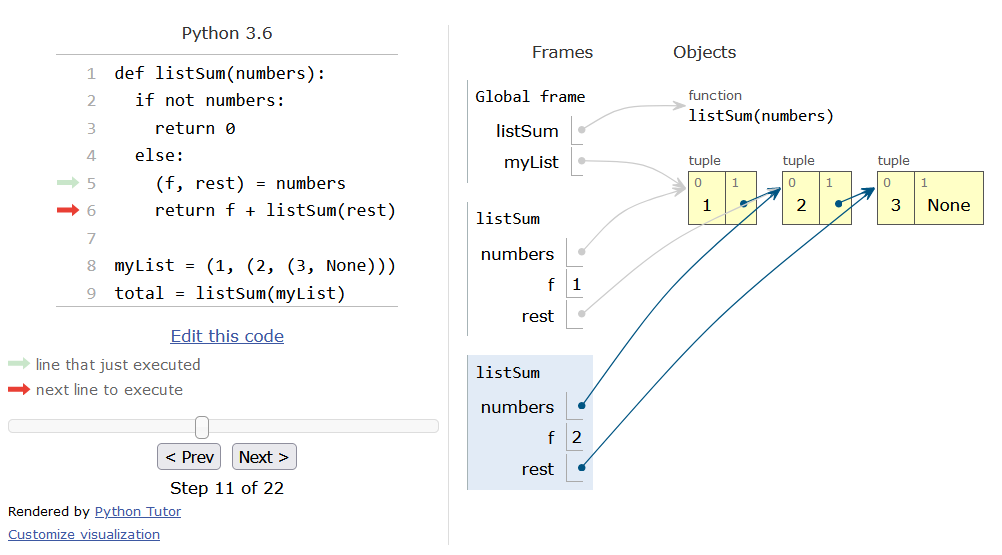
\includegraphics[width=\textwidth]{chapter2/pythontutor.png}
  \caption{Visualisasi Eksekusi Kode pada Python Tutor \\ Sumber: \textcite{guo2013pythontutor}} \label{fig:pythontutor}
\end{figure}

\begin{figure}[H]
  \centering
  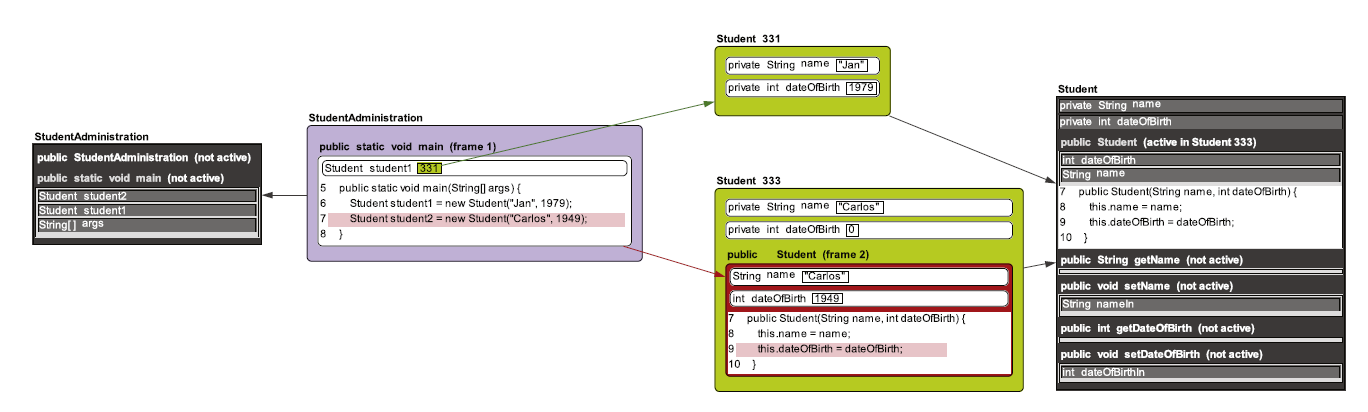
\includegraphics[width=\textwidth]{chapter2/evizor.png}
  \caption{Visualisasi Eksekusi Kode pada EVIZOR \\ Sumber: \textcite{moons2013pilot}} \label{fig:evizor}
\end{figure}

\subsubsection{Ragam Implementasi ILE} \label{sssec:ragam-implementasi-ile}
Pembelajaran pemrograman secara daring saat ini menggunakan berbagai macam media dalam penyampaian materinya. Mulai dari berbentuk teks, video, animasi, \textit{mentoring}, \textit{bootcamp}, \textit{webinar}, latihan soal, hingga simulasi berbentuk gamifikasi seperti pada \textcite{codingame2021media} yang dapat dilihat pada \autoref{fig:codingame}. Seiring dengan bertambahnya kompetitor, beragam situs mulai mengadopsi sistem pembelajaran yang lebih interaktif, mudah dipahami, dan menyenangkan agar membedakan dengan kompetitor lainnya dan menjadi nilai tambah bagi penggunanya.

\begin{figure}[H]
  \centering
  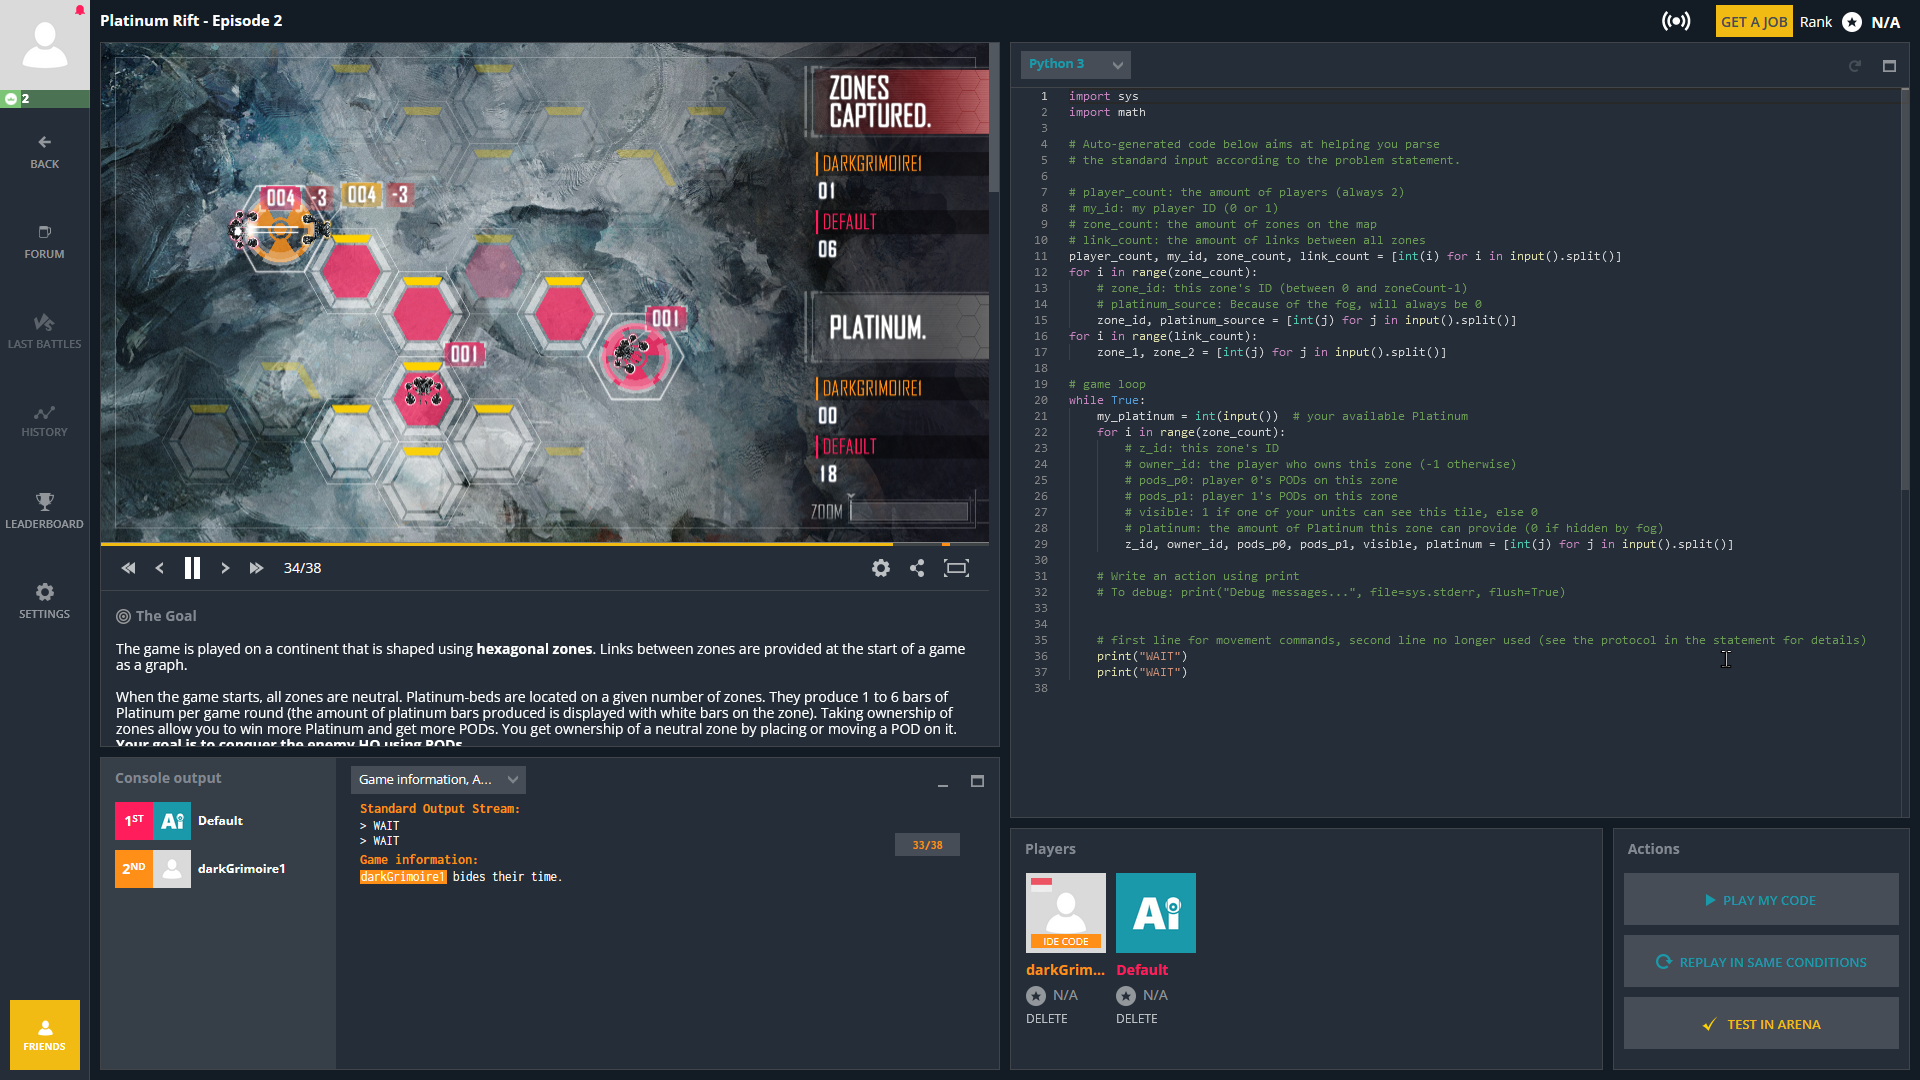
\includegraphics[width=0.8\textwidth]{chapter2/codingame.png}
  \caption{\label{fig:codingame}Gamifikasi pada \href{https://www.codingame.com}{CodinGame} \\ Sumber: \textcite{codingame2021media}}
\end{figure}

\textcite{sololearn2021media} menggunakan materi berbentuk teks yang disertai latihan soal pemrograman berbentuk pilihan ganda, isian singkat, serta \textit{drag \& drop} jawaban pada tempat yang telah disediakan. \href{https://www.sololearn.com}{Sololearn} juga memiliki Web IDE yang dapat dipakai oleh penggunanya untuk mengerjakan soal latihan pemrograman seperti pada \autoref{fig:sololearn}. \href{https://www.sololearn.com}{Sololearn} berfokus terhadap latihan implementasi program secara langsung dan mempelajari berbagai macam fitur dan logika dalam bahasa tersebut.

\begin{figure}[H]
  \centering
  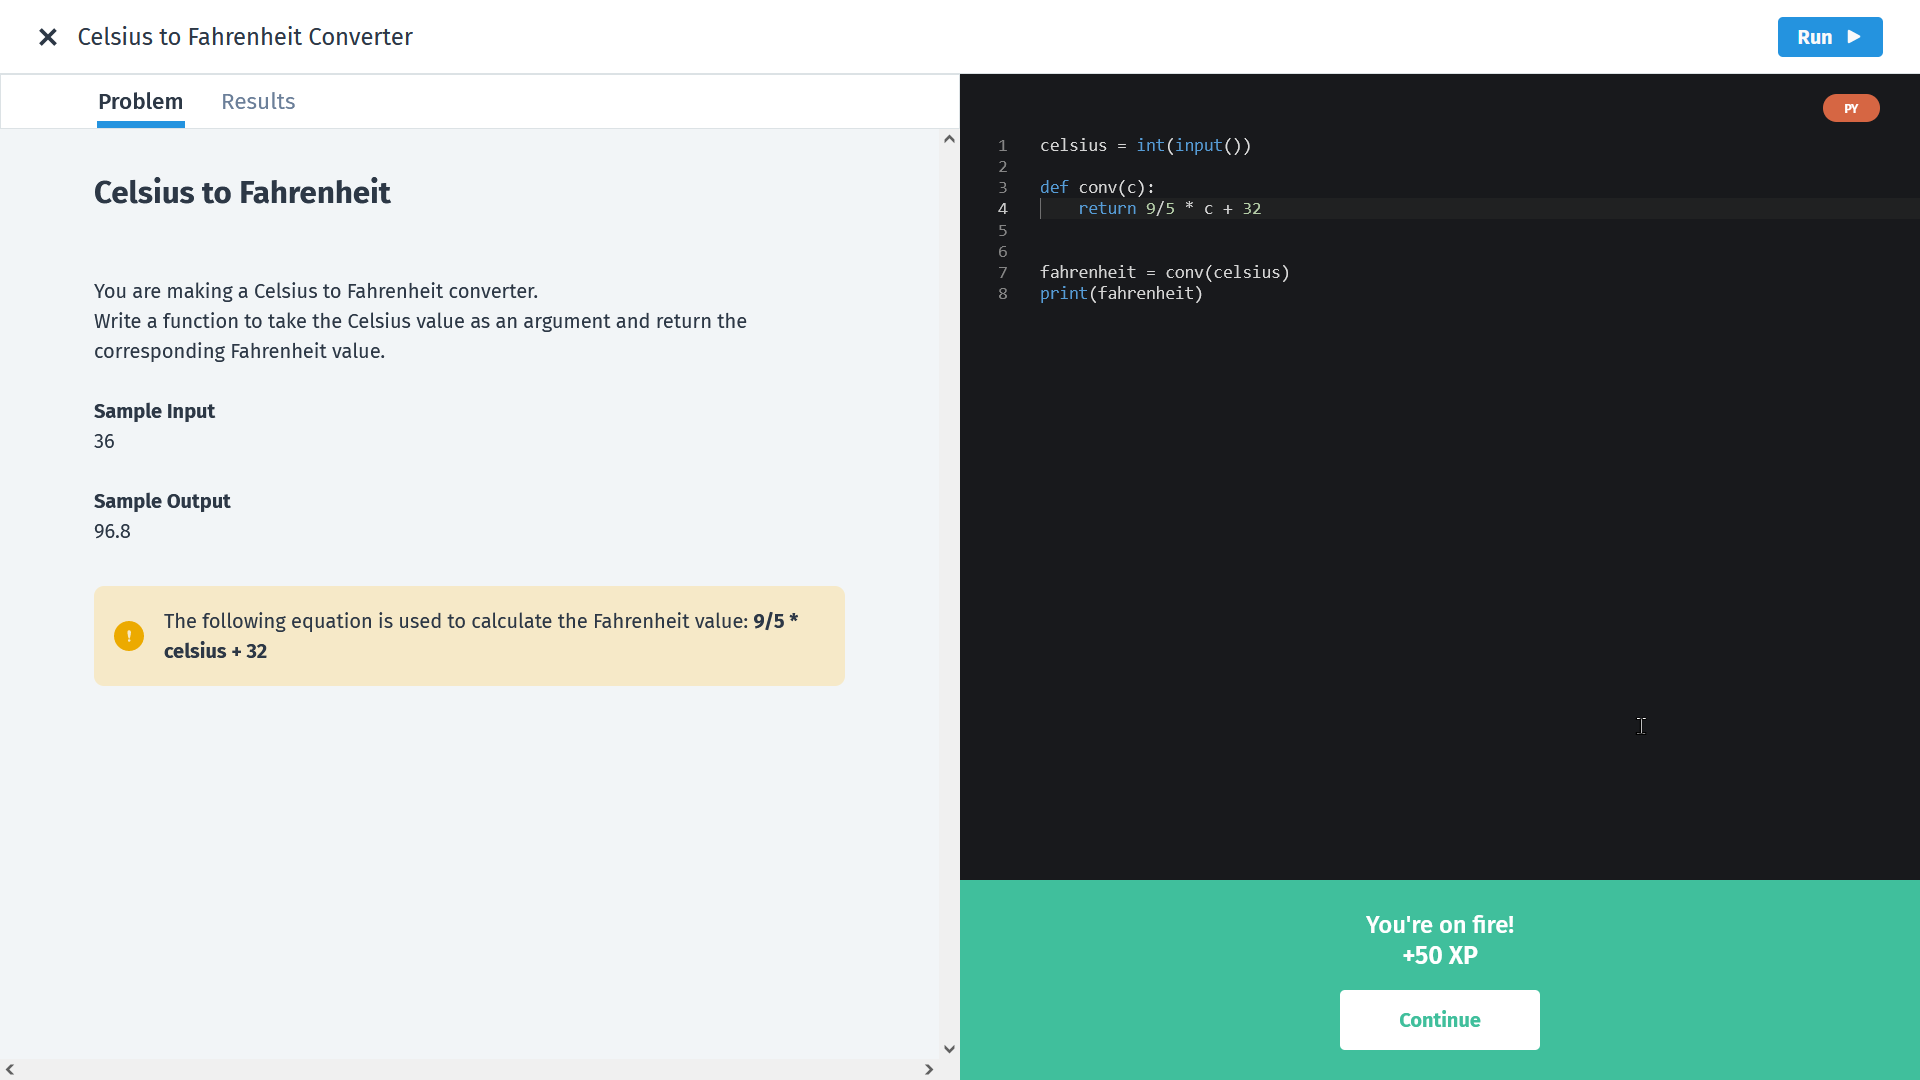
\includegraphics[width=0.8\textwidth]{chapter2/sololearn.png}
  \caption{\label{fig:sololearn}Belajar dengan latihan soal pada \href{https://www.sololearn.com}{Sololearn} \\ Sumber: \textcite{sololearn2021media}}
\end{figure}

Sementara itu, \href{https://brilliant.org}{Brilliant} menggunakan teknik yang berbeda. \textcite{brilliant2021media} memakai eksekusi pemrograman yang lebih visual dan interaktif sehingga membuat pembelajaran lebih menarik dan menyenangkan (contoh pada \autoref{fig:brilliant}). \href{https://brilliant.org}{Brilliant} juga menggunakan berbagai macam visual pendukung seperti animasi dan grafis yang menarik dan mudah dipahami, serta juga menggunakan bahasa yang dinarasikan sedemikian rupa sehingga konsep pemrograman yang rumit menjadi mudah dipahami.

\begin{figure}[H]
  \centering
  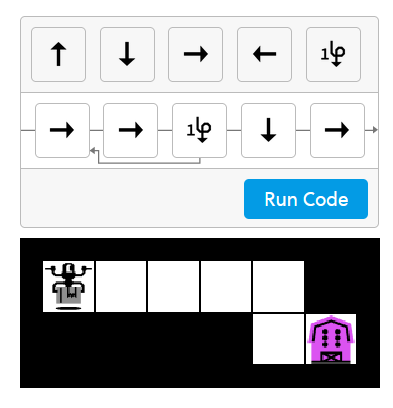
\includegraphics[width=0.3\textwidth]{chapter2/brilliant.png}
  \caption{\label{fig:brilliant}Salah satu pembelajaran interaktif pada \href{https://brilliant.org}{Brilliant} \\ Sumber: \textcite{brilliant2021media}}
\end{figure}

Selain dari \href{https://www.sololearn.com}{Sololearn} dan \href{https://brilliant.org}{Brilliant}, terdapat juga platform-platform lainnya seperti \href{https://www.katacoda.com/}{Katacoda} \parencite{katacoda2021media} yang menyediakan kelas pemrograman interaktif menggunakan Web IDE sebagai metode penyampaian materi utama dan instruksi dalam bentuk teks sehingga pengguna langsung dapat terjun mempelajari dan mencoba materi yang diberikan. Katacoda juga menyediakan seluruh kelasnya secara gratis untuk siapapun. Pendekatan seperti Katacoda juga dapat kita lihat pada platform lain seperti \href{https://www.codesaya.com/}{CodeSaya} \parencite{codesaya2021media}. Platform-platform ini menggunakan teks sebagai hasil feedback eksekusi kode. Contoh tampilan Web IDE Katacoda dan CodeSaya dapat dilihat pada \autoref{fig:katacoda} dan \autoref{fig:codesaya}.

\begin{figure}[H]
  \centering
  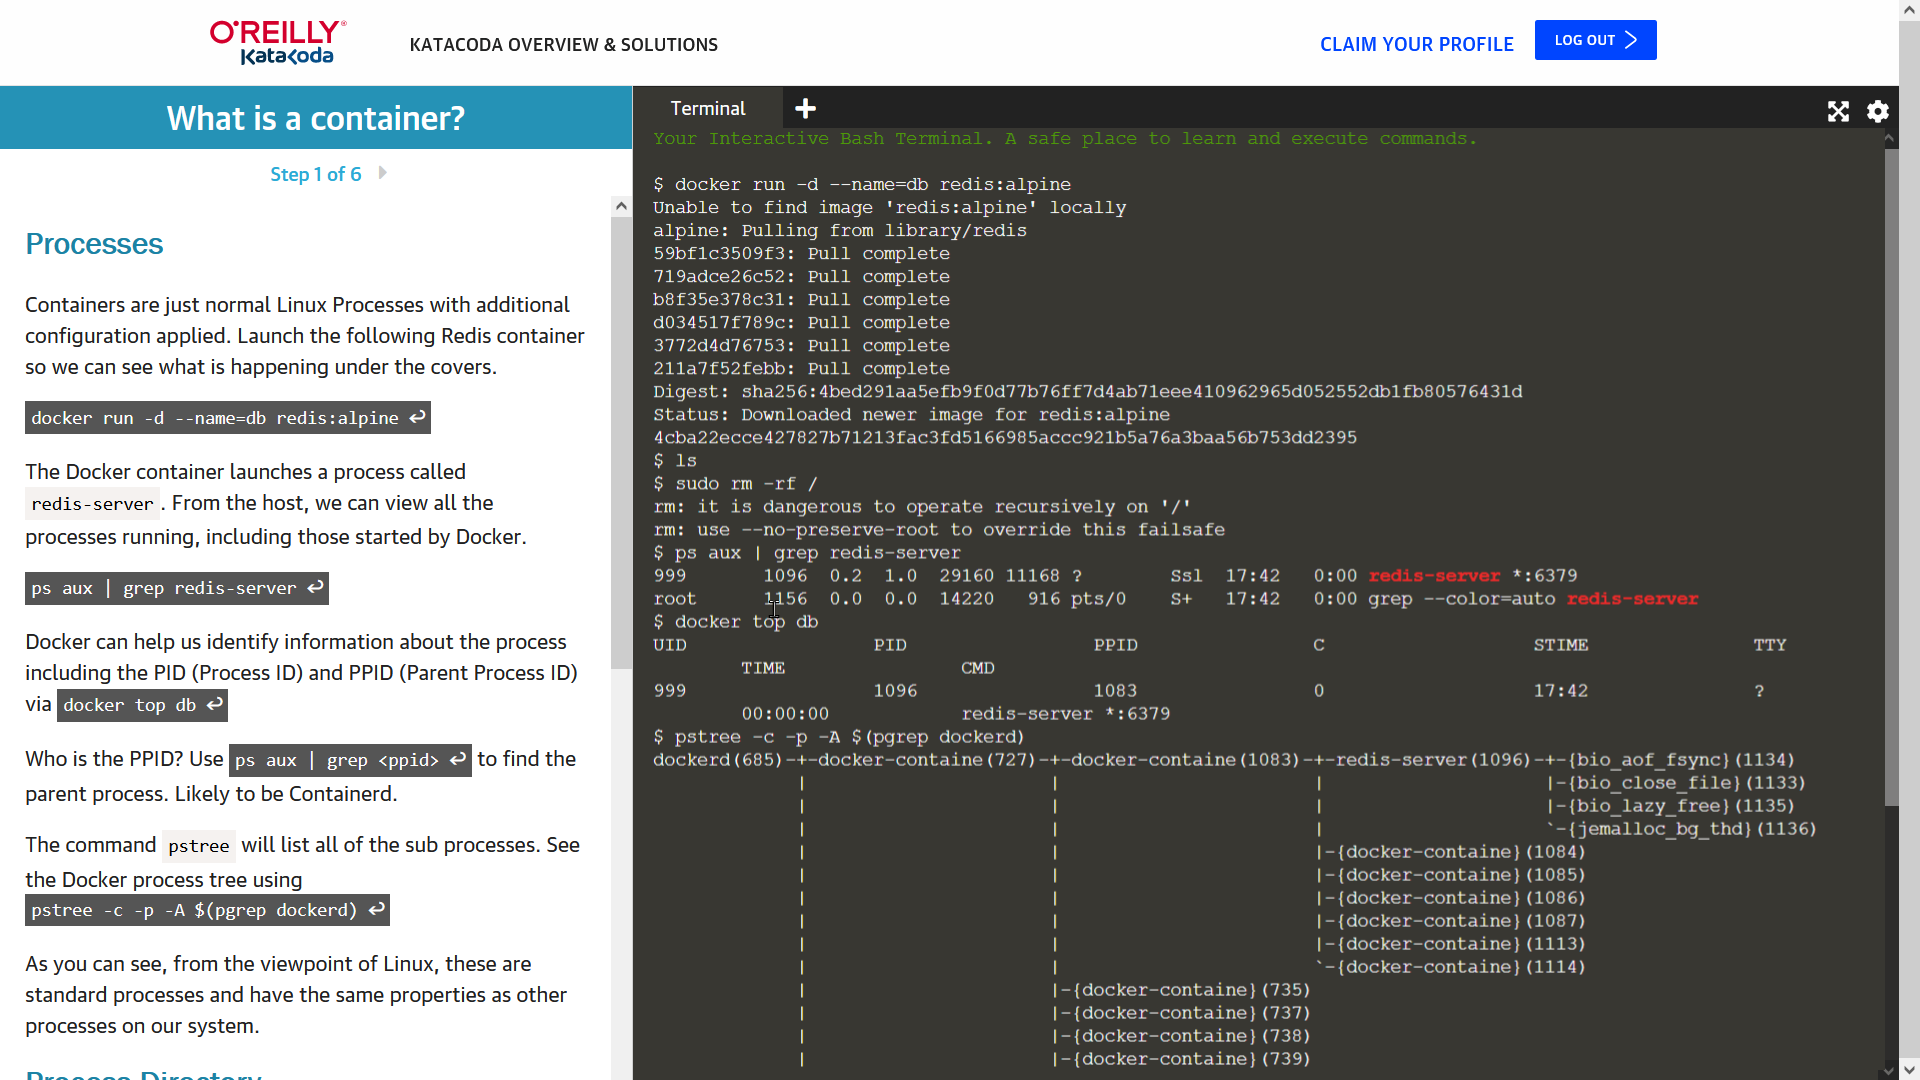
\includegraphics[width=0.8\textwidth]{chapter2/katacoda.png}
  \caption{\label{fig:katacoda}Terminal interaktif pada kelas Docker di \href{https://www.katacoda.com/}{Katacoda} \\ Sumber: \textcite{katacoda2021media}}
\end{figure}

\begin{figure}[H]
  \centering
  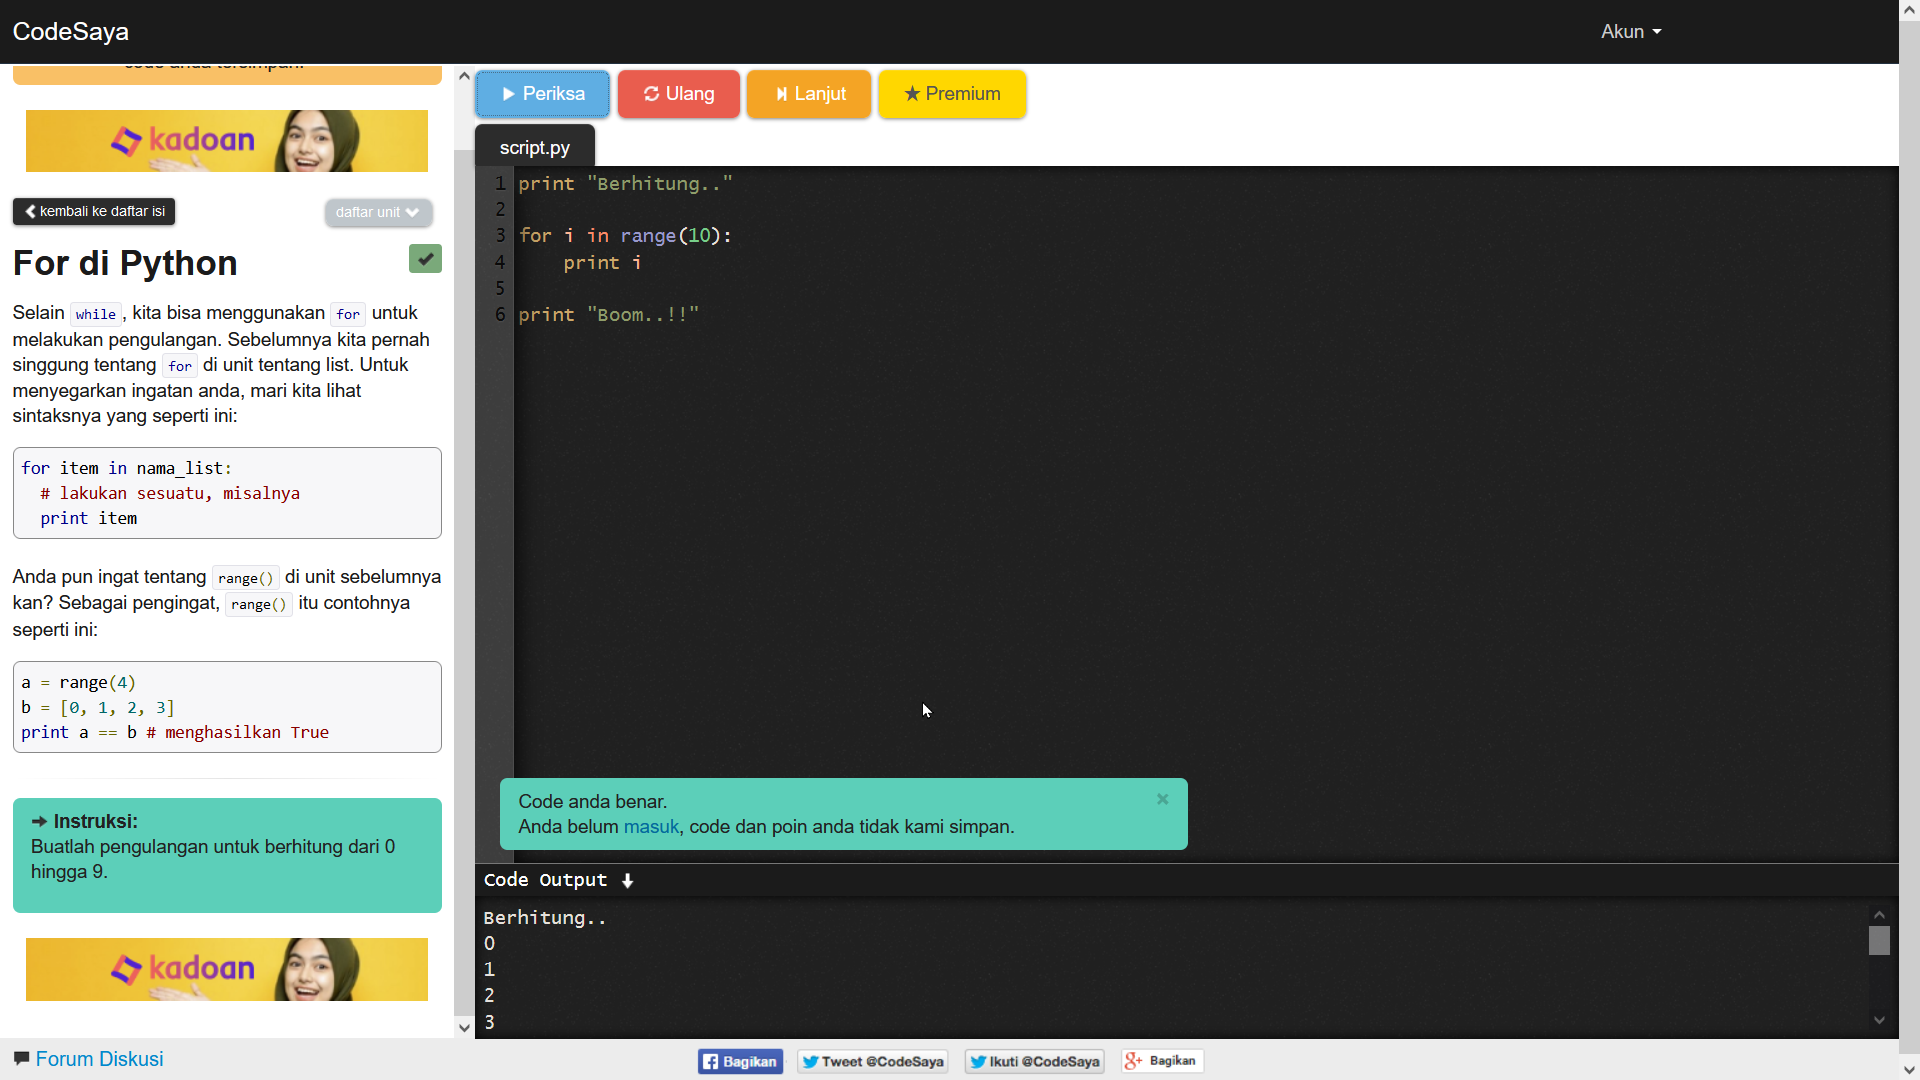
\includegraphics[width=0.8\textwidth]{chapter2/codesaya.png}
  \caption{\label{fig:codesaya}Contoh konten kelas pada \href{https://www.codesaya.com/}{CodeSaya} \\ Sumber: \textcite{codesaya2021media}}
\end{figure}

Mirip dengan \href{https://www.katacoda.com/}{Katacoda} yang metode utama pembelajaran menggunakan Web IDE, terdapat juga \href{https://flexboxfroggy.com/}{Flexbox Froggy} \parencite{froggy2021media} beserta permainan lainnya dari \href{https://codepip.com/games/}{Codepip} yang memiliki hasil feedback eksekusi kode secara visual seperti pada \autoref{fig:froggy}. \href{https://flexboxfroggy.com/}{Flexbox Froggy} menggunakan feedback visual sehingga hasil \textit{style CSS} yang dibuat dapat langsung terlihat oleh pengguna dan disesuaikan agar dapat memenuhi tujuan yang diinginkan selama mengerjakan latihan. Integrasi pembelajaran dengan gamifikasi visual membuat pembelajaran lebih interaktif.

\begin{figure}[H]
  \centering
  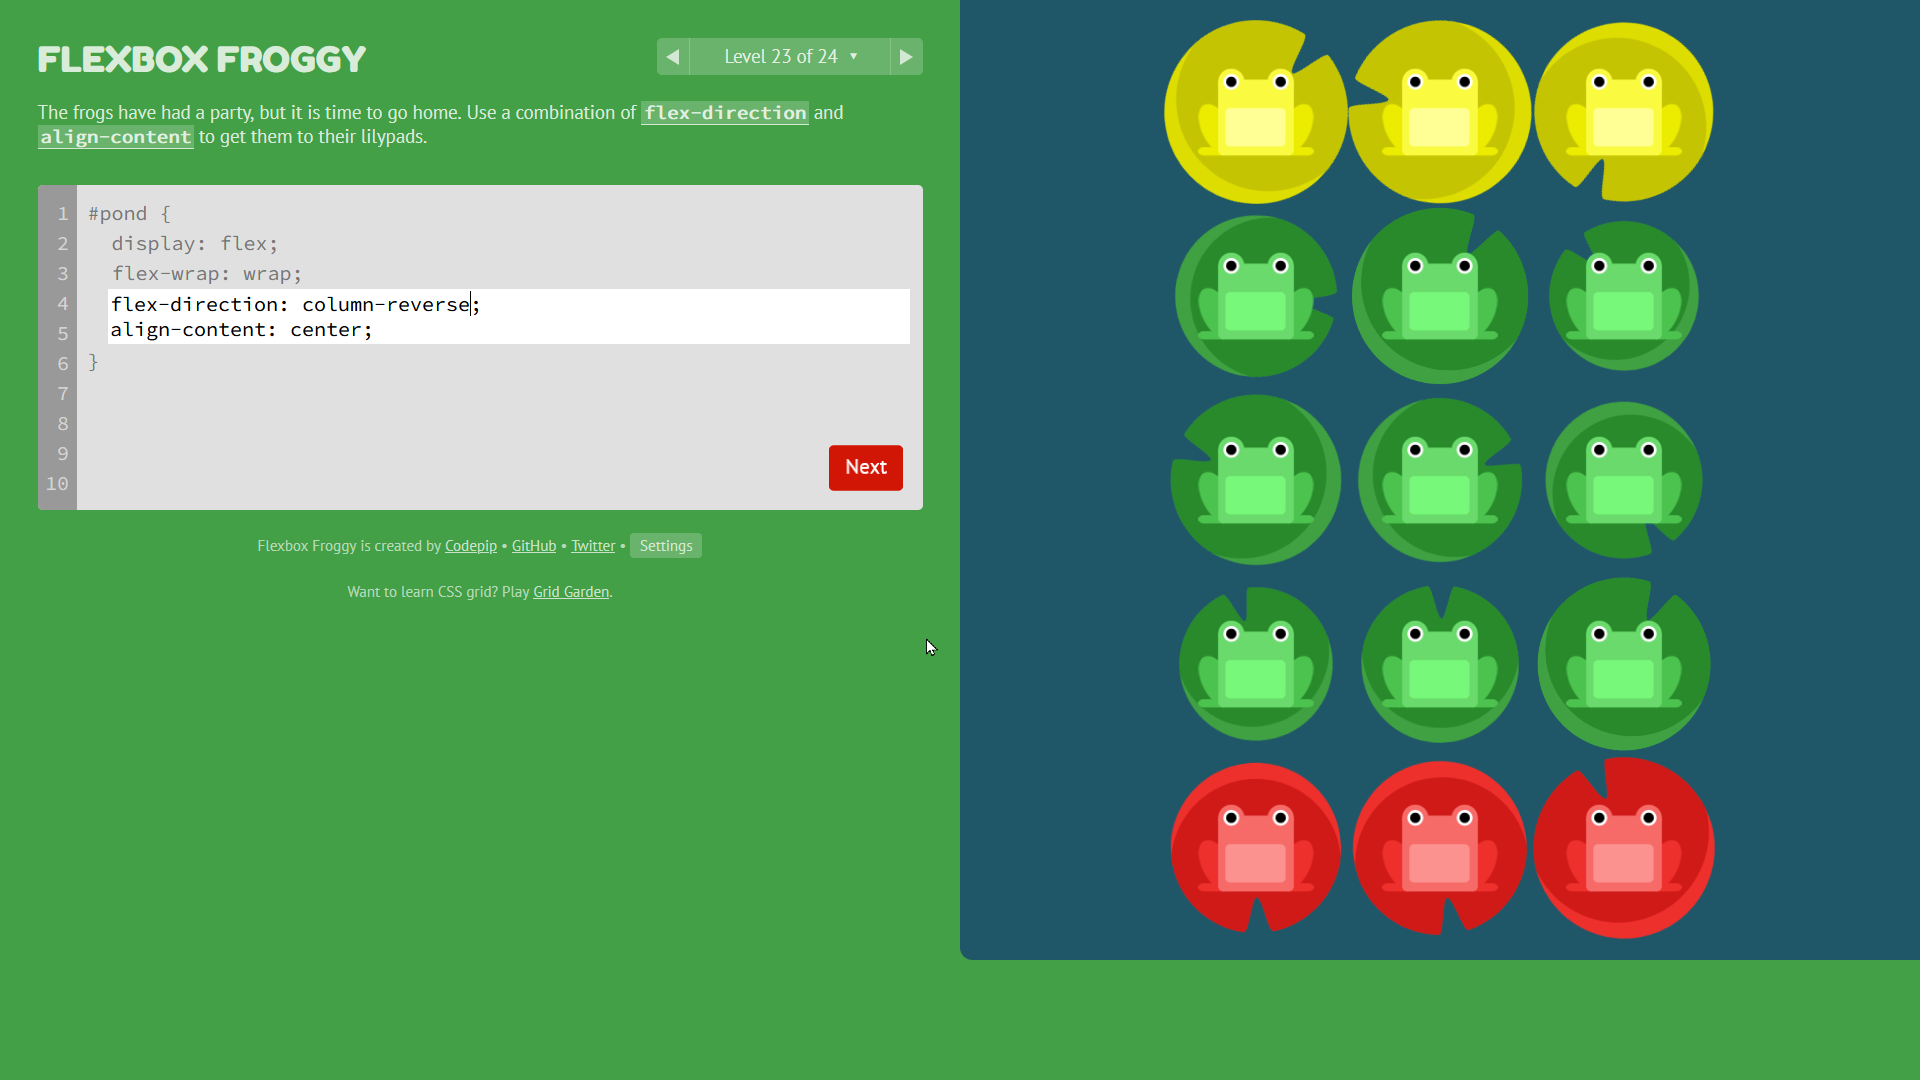
\includegraphics[width=0.8\textwidth]{chapter2/froggy.png}
  \caption{Visualisasi penggunaan flexbox di \href{https://www.flexboxfroggy.com/}{Flexbox Froggy} \\ Sumber: \textcite{froggy2021media}} \label{fig:froggy}
\end{figure}

Terdapat banyak platform pembelajaran pemrograman secara daring yang mengintegrasikan permainan ke dalam metode pembelajarannya, baik itu melalui latihan praktiknya, penjelasan materinya, hingga sistem pengembangan diri pada platform itu sendiri. Salah satu platform yang memiliki ketiganya adalah \textcite{progate2021media} yang menarasikan materi menggunakan maskot serta cerita yang mudah dipahami (lihat \autoref{fig:progate-materi}), latihan praktik yang langsung terjun implementasi (lihat \autoref{fig:progate-soal}), serta sistem level dan \textit{achievement/badges} bagi pengguna yang aktif menggunakan platformnya.

\begin{figure}[H]
  \centering
  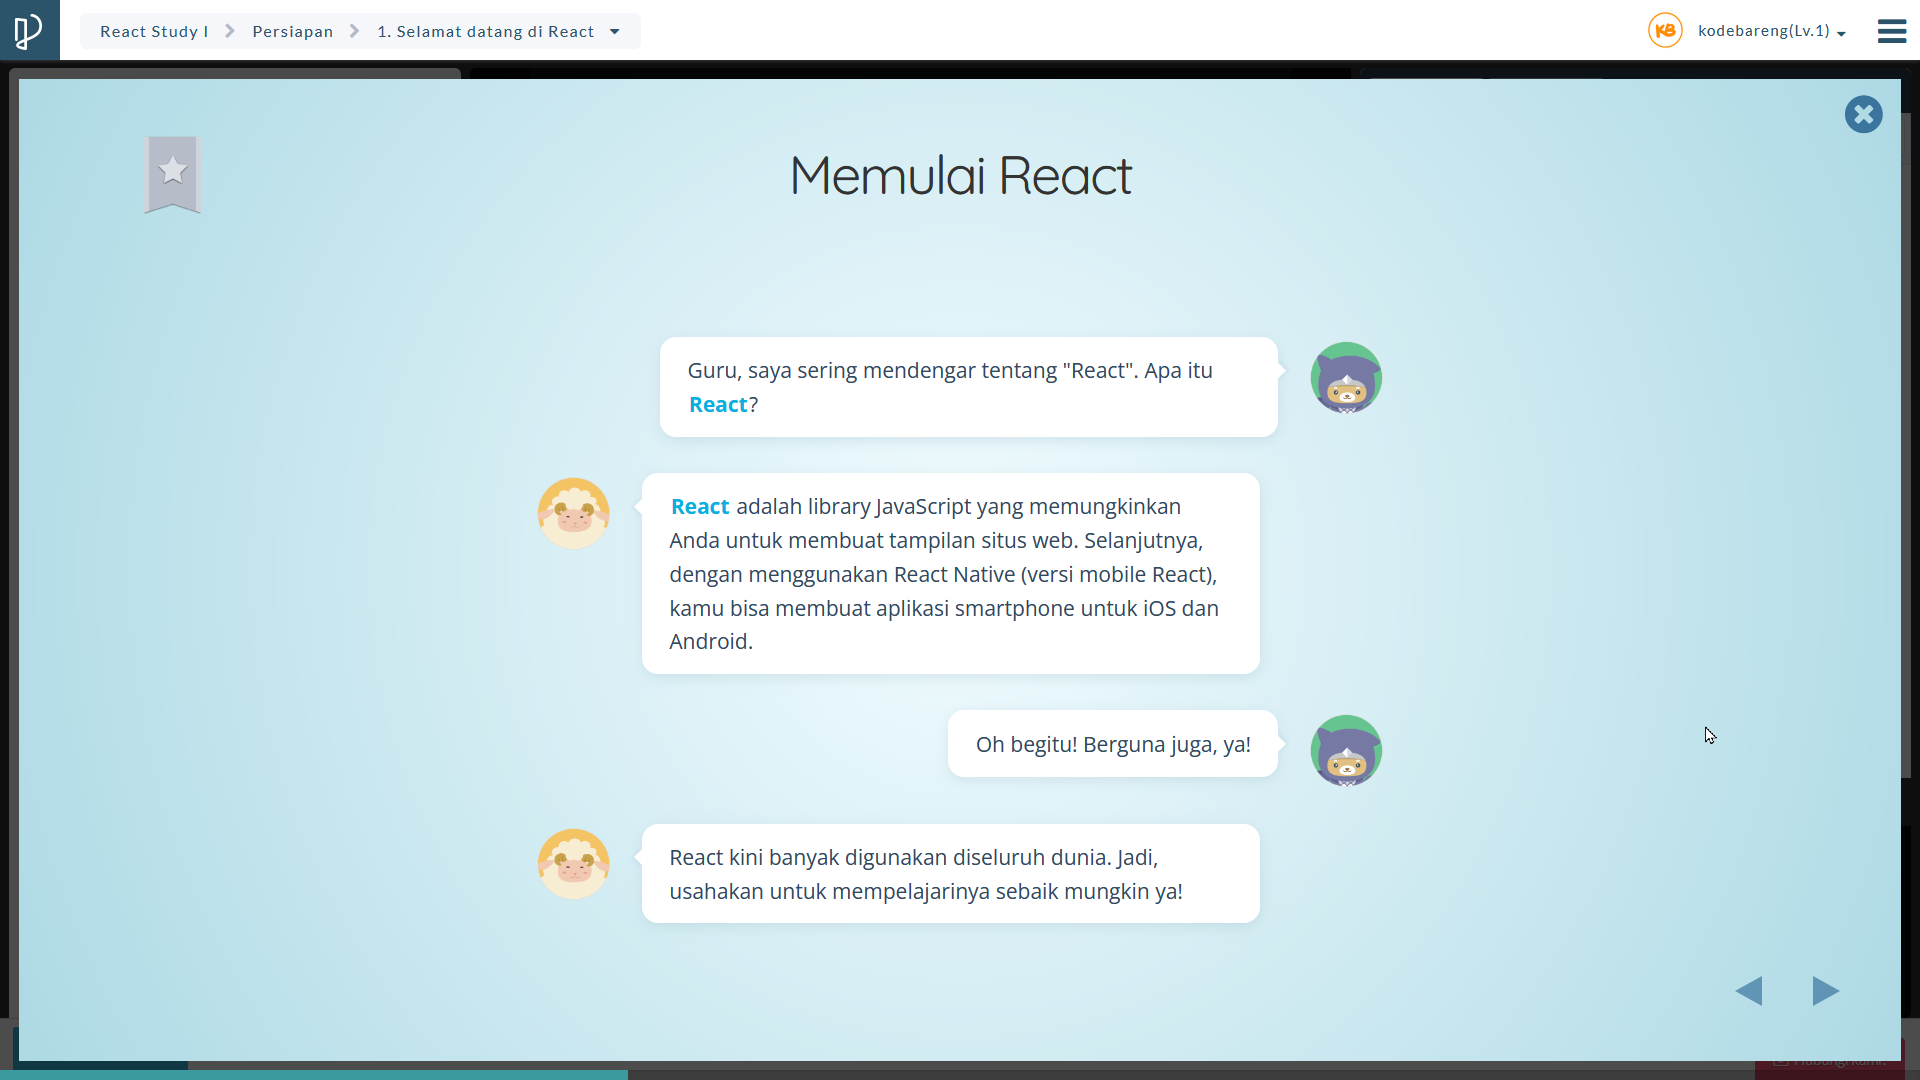
\includegraphics[width=0.8\textwidth]{chapter2/progate-intro.png}
  \caption{Penyampaian materi pada \href{https://www.progate.com/}{Progate} \\ Sumber: \textcite{progate2021media}} \label{fig:progate-materi}
\end{figure}

\begin{figure}[H]
  \centering
  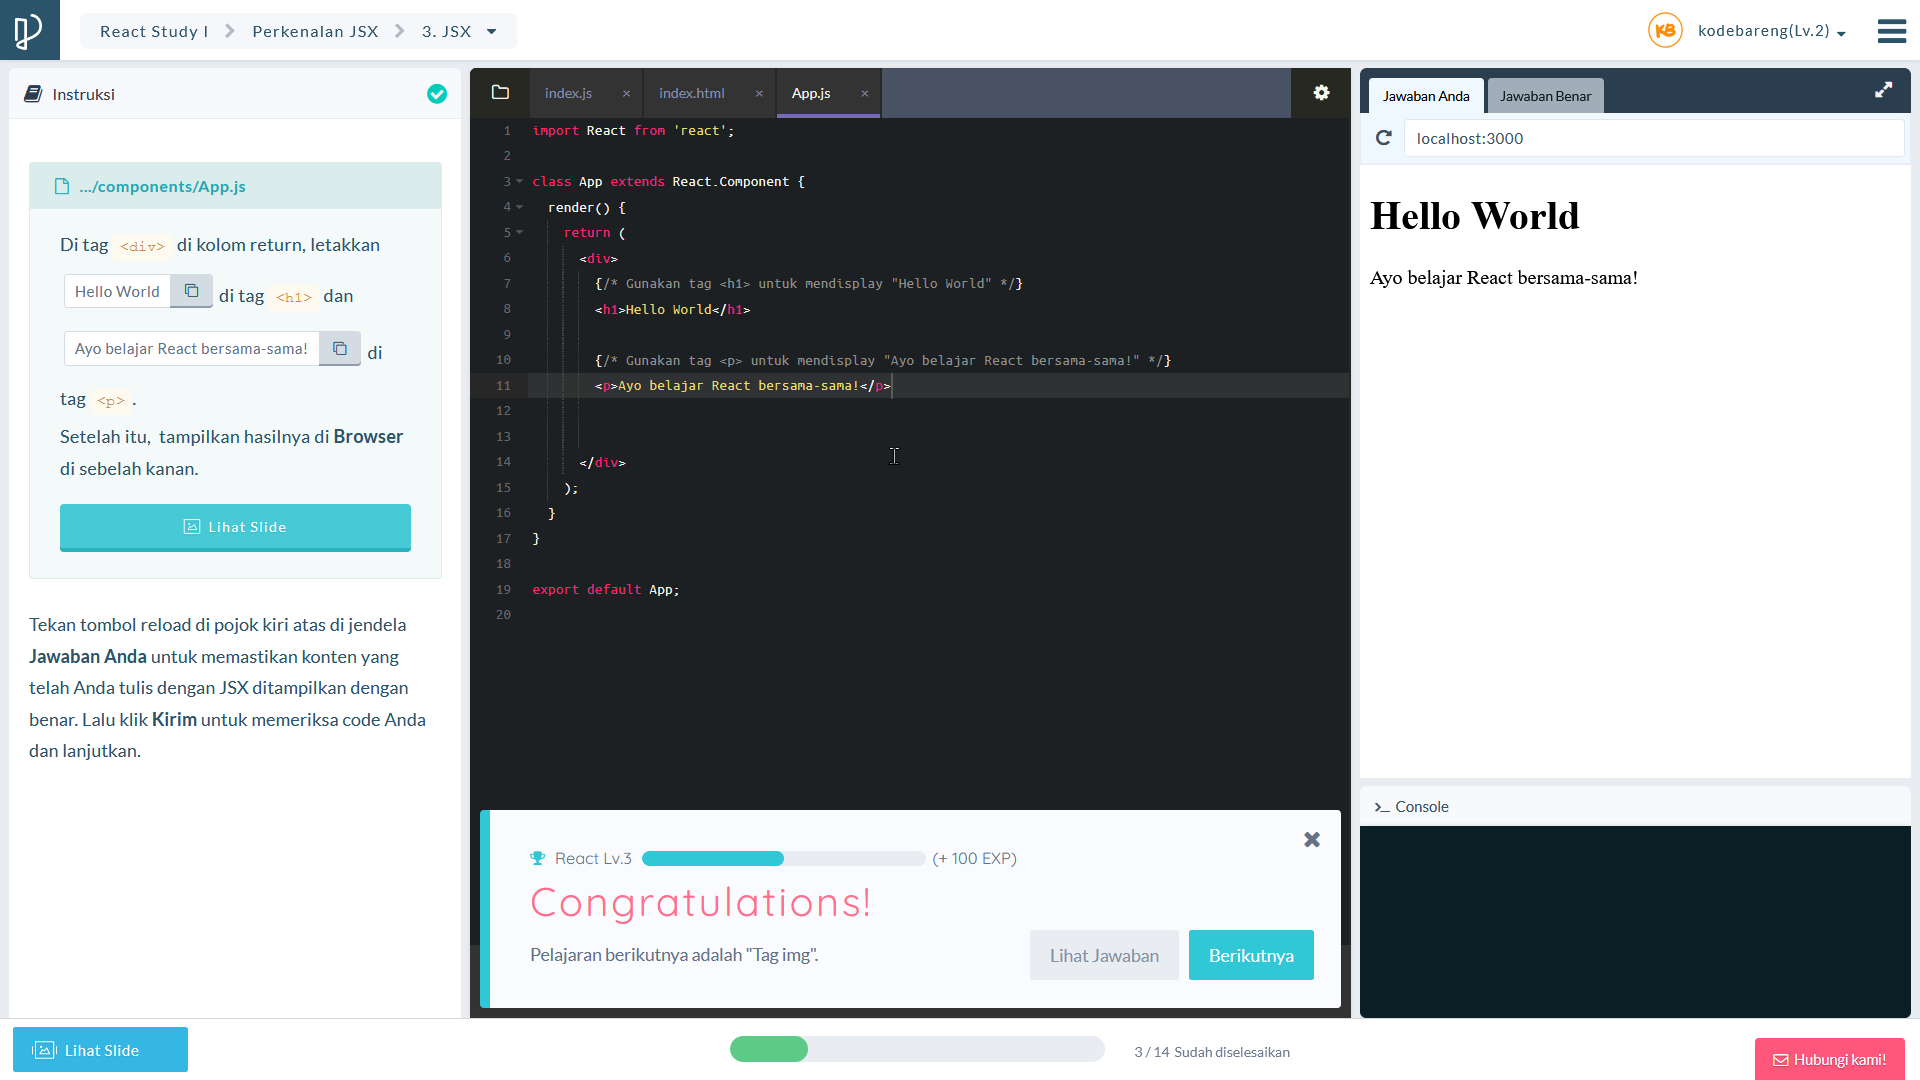
\includegraphics[width=0.8\textwidth]{chapter2/progate-code.png}
  \caption{Latihan implementasi pada \href{https://www.progate.com/}{Progate} \\ Sumber: \textcite{progate2021media}}\label{fig:progate-soal}
\end{figure}

Manfaat interaktivitas digital dalam pembelajaran pemrograman masih menjadi topik hangat di kalangan peneliti. Salah satu studi terkait pembelajaran interaktif terminal UNIX uAssign \parencite{bailey2019uassign} memberikan konklusi bahwa pembelajaran interaktif menggunakan uAssign menghasilkan peningkatan di kemampuan menggunakan terminal siswa yang menggunakannya, terutama bagi siswa yang belum mengetahui  penggunaan terminal. Studi lain pada \href{https://pythontutor.com}{Online Python Tutor} \parencite{guo2013pythontutor}---aplikasi web yang memberikan visualisasi eksekusi kode Python---menjelaskan bahwa visualisasi yang disediakan oleh \href{https://pythontutor.com}{Online Python Tutor} sangat membantu dalam proses pembelajaran. Eksekusinya yang dilakukan secara daring juga memudahkan siswa dalam menggunakan aplikasi tersebut pada forum pembelajaran untuk membantu siswa lain dalam memecahkan permasalahan, tanpa harus melakukan instalasi ataupun konfigurasi terlebih dahulu. Terdapat juga IDEOL \parencite{tran2013interactive} yaitu Web IDE yang berfokus pada aspek kolaboratif secara \textit{real-time} dan menyediakan wadah berdiskusi antara pemakainya sehingga dapat mempermudah proses \textit{debugging} dan pembagian tugas antar anggota kelompok karena kode selalu sinkron dengan anggota kelompok lain.

\section{Pemahaman Konsep Pemrograman}
Menurut \textcite{mayer1981psychology}, terdapat 2 metode dalam mempelajari cara memecahkan suatu masalah: menghafal (\textit{rote learning}) atau memahami (\textit{understanding}). Metode pembelajaran dengan menghafal artinya pelajar memecahkan suatu masalah dengan menghafal cara atau prosedur memecahkan spesifik persoalan tersebut, misalnya dengan menghafal rumus. Sementara, metode pembelajaran dengan memahami artinya pelajar memecahkan suatu masalah dengan memahami apa yang perlu dilakukan untuk mencapai solusi dari permasalahan tersebut. Hal tersebut diilustrasikan dengan seorang pelajar yang memecahkan persoalan geometri menggunakan rumus (menghafal), dibandingkan dengan seorang pelajar yang memecahkan persoalan geometri dengan mengetahui cara menyederhanakan bangun ruang tersebut menjadi bangun sederhana seperti persegi (memahami). Kedua metode dapat memecahkan permasalahan yang sama, namun apabila diberikan permasalahan yang baru, maka pelajar yang memakai metode memahami akan dapat menjawab persoalan tersebut. Hal ini disebabkan karena pelajar dengan metode menghafal tidak dapat mentransfer/menerapkan ilmunya pada permasalahan yang baru. Maka dari itu, pemahaman konsep merupakan salah satu faktor yang penting dalam pembelajaran karena dengan memahami konsep, pelajar dapat memahami situasi persoalan yang baru sehingga dapat membuat solusi yang benar.

Terdapat 2 taksonomi yang biasa digunakan dalam membuat dan menilai pembelajaran, yaitu taksonomi Bloom dan taksonomi SOLO (\textit{Structure of Observed Learning Outcomes}). Taksonomi Bloom adalah taksonomi yang mengkategorikan pembelajaran berdasarkan pada tingkat kesulitan dan kekhususan (\textit{specificity}) suatu persoalan secara kognitif \parencite{woolfolk2016educational}, sementara taksonomi SOLO adalah taksonomi yang mengkategorikan pembelajaran berdasarkan tahapan pemahaman pelajar dalam mempelajari suatu materi atau persoalan \parencite{biggs2014evaluating}. Dalam mengukur pemahaman pelajar, taksonomi SOLO lebih tepat digunakan karena taksonomi SOLO dapat mengukur pemahaman pelajar berdasarkan respon pelajar dari suatu permasalahan, sementara taksonomi Bloom mengukur pemahaman pelajar berdasarkan bisa atau tidaknya pelajar menjawab suatu pertanyaan pada level tertentu.

Dalam taksonomi SOLO, terdapat 5 level pemahaman pelajar \parencite{biggs2014evaluating} yang dinamakan SOLO Level yang dapat dilihat pada \autoref{tab:solo-level}. SOLO Level dapat digunakan untuk mengukur pemahaman pelajar dalam mempelajari suatu materi atau persoalan dengan mempelajari respon pelajar terhadap persoalan yang diberikan.

\small
\begin{longtable}[c]{|l|l|>{\setlength{\baselineskip}{0.75\baselineskip}}p{0.5\linewidth}|}
  \caption{Kategori penilaian SOLO Level} \label{tab:solo-level}                                                                                              \\ \hline
  \rowcolor{gray!30}
  \textbf{SOLO Level} & \textbf{Kategori} & \textbf{Deskripsi}                                                                                                \\ \hline
  \endfirsthead
  %
  \caption*{\autoref{tab:solo-level} (lanjutan): Kategori penilaian SOLO Level}                                                                               \\ \hline
  \rowcolor{gray!30}
  \textbf{SOLO Level} & \textbf{Kategori} & \textbf{Deskripsi}                                                                                                \\ \hline
  \endhead
  %
  1                   & Prestructural     & Memperlihatkan kurangnya pengetahuan pada domain tersebut atau tidak berhubungan dengan pertanyaan yang diberikan \\ \hline
  2                   & Unistructural     & Terdapat pemahaman terkait satu konsep pembelajaran, namun tidak berhubungan dengan pertanyaan yang diberikan     \\ \hline
  3                   & Multistructural   & Terdapat pemahaman terkait beberapa konsep pembelajaran, namun tidak saling berkaitan                             \\ \hline
  4                   & Relational        & Terdapat pemahaman beberapa konsep pembelajaran dan saling berkaitan                                              \\ \hline
  5                   & Extended Abstract & Pemahaman telah digeneralisir agar dapat ditransfer pada domain pembelajaran lainnya                              \\ \hline
\end{longtable}
\normalsize

\section{Platform Kodebareng}

Kodebareng merupakan platform pembelajaran pemrograman berbahasa Indonesia yang mengintegrasikan pembelajaran dengan gamifikasi dan pembelajaran yang interaktif sehingga pembelajaran akan menjadi lebih mudah dan menyenangkan. Situs Kodebareng adalah aplikasi yang dibuat oleh tim diginove "Kodebareng" yang berfungsi untuk mengajarkan pemrograman. Kodebareng ditujukan bagi pelajar SMA hingga awal perkuliahan yang memiliki keinginan untuk mulai mempelajari pemrograman dan belum memiliki dasar pemrograman sebelumnya. Sebelum Tugas Akhir ini, KodeBareng baru memiliki MVP berupa Landing Page, profil akun sederhana, serta demo kelas pemrograman Python yang dapat diakses kontennya berupa teks, kuis, serta latihan pemrograman dengan autograder sederhana. Contoh tampilan Kodebareng dapat dilihat pada \autoref{fig:kodebareng-tampilan}.

\begin{figure}[H]
  \centering
  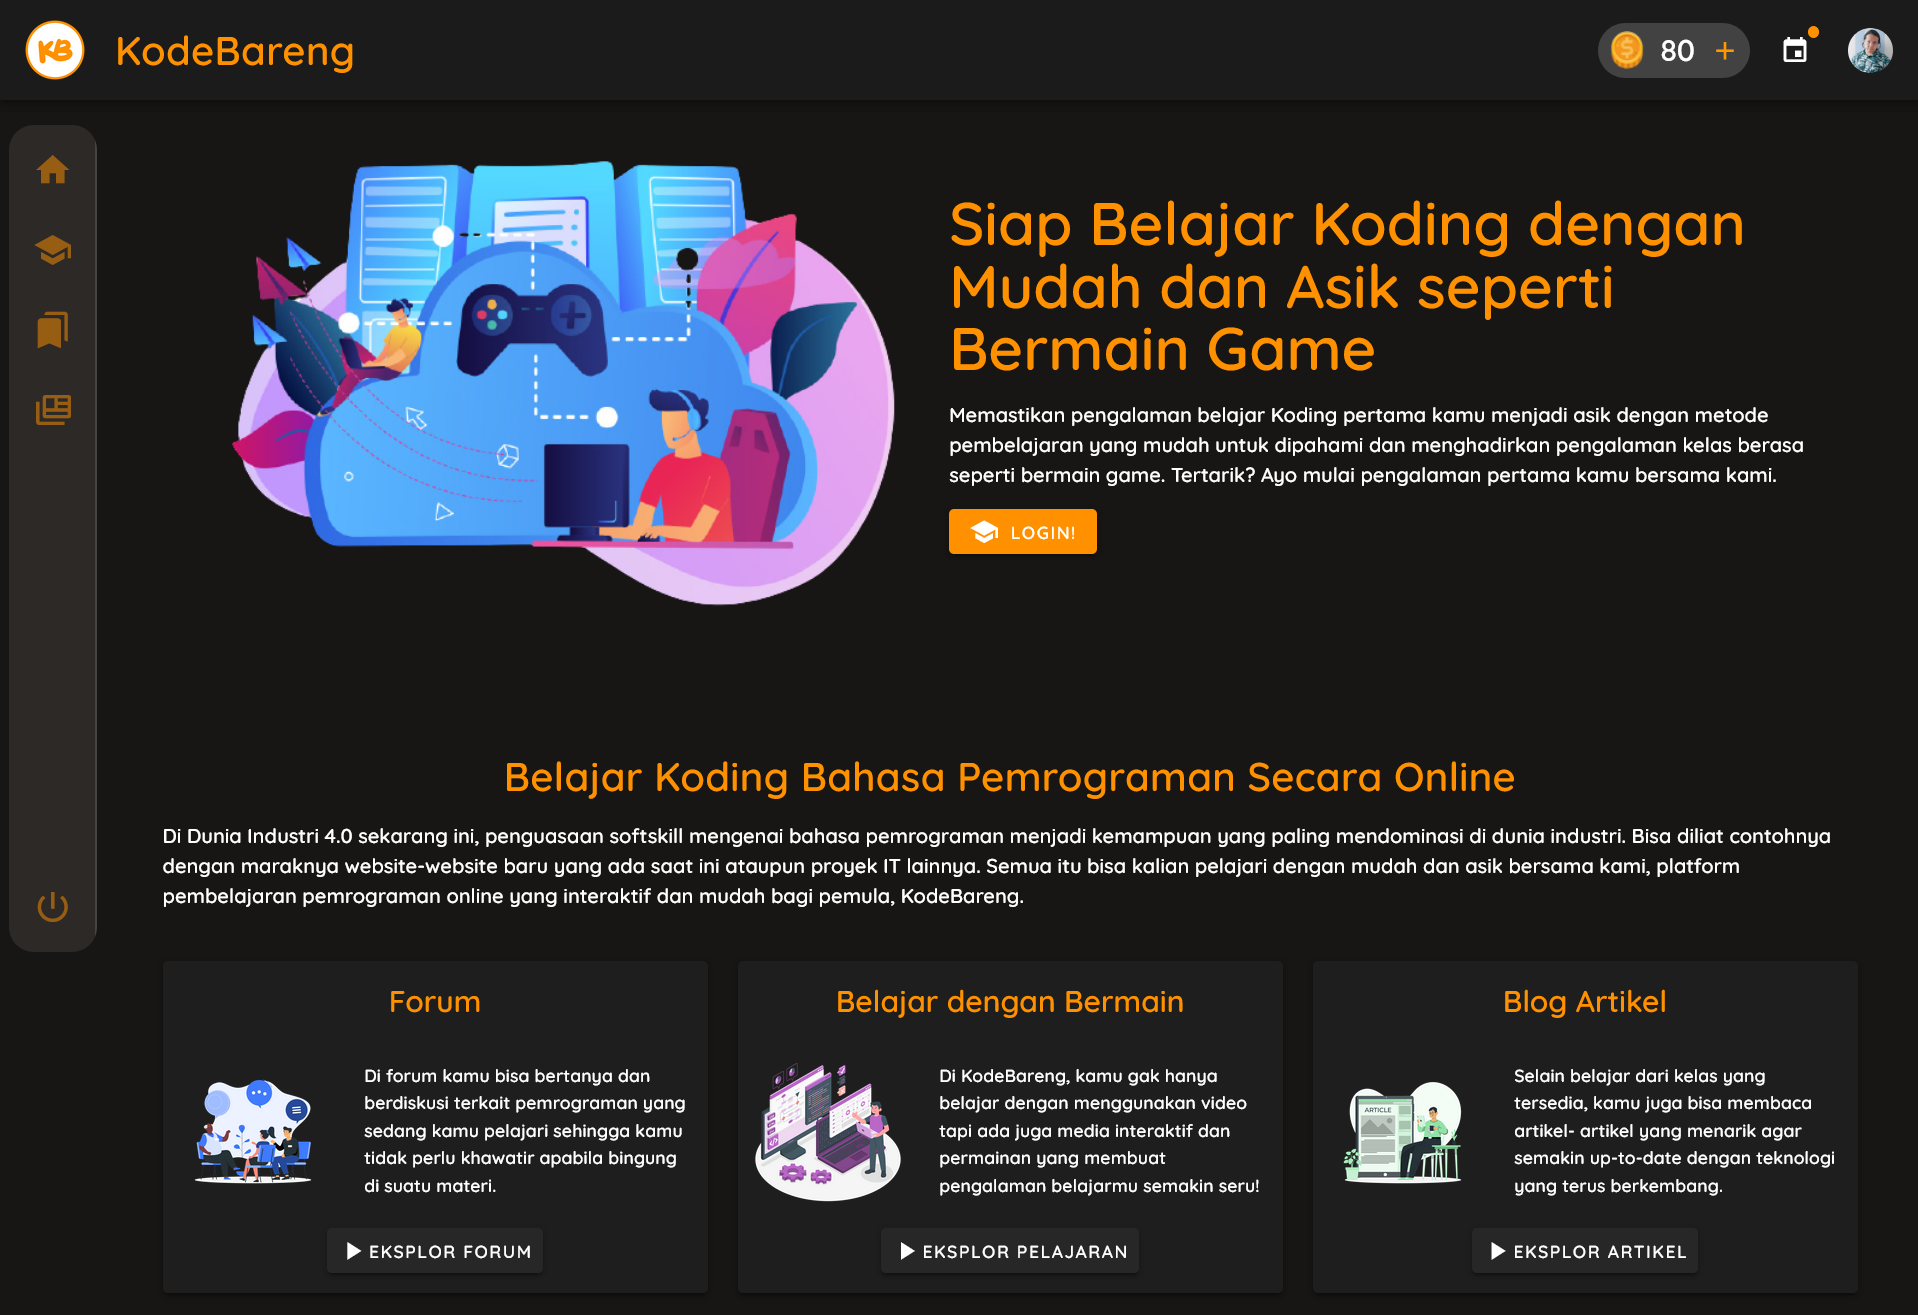
\includegraphics[width=0.6\textwidth]{chapter2/kodebareng.png}
  \caption{Tampilan di Kodebareng \\ Sumber: Penulis (2022)}\label{fig:kodebareng-tampilan}
\end{figure}

Pembelajaran pada KodeBareng terfokus pada kelas-kelas pemrograman. Setiap kelas memiliki beberapa modul (diibaratkan sebagai bab dalam buku), dan setiap modul memiliki beberapa \textit{stage} (diibaratkan sebagai subbab dalam buku). Pembelajaran pada KodeBareng dapat dibagi menjadi 2, yaitu pembelajaran melalui materi (seperti pada ) dan pembelajaran dengan latihan soal. KodeBareng sendiri termasuk dalam pendekatan belajar "melalui" pembelajaran interaktif sesuai dengan definisi pada \textcite{reeves2012interactive} karena interaktivitasnya masih terletak pada materi dan pembawaannya.

Materi pembelajaran pada KodeBareng dibawakan dalam bentuk teks dan gambar visual, sementara contoh kode diberikan secara teks yang mengandung kode, masukan (\textit{input}), dan keluaran (\textit{output}) seperti yang dapat dilihat pada \autoref{fig:kodebareng-materi}. Setelah pelajar mempelajari materi pada suatu \textit{stage}, pelajar dapat menekan tombol "Done" untuk melanjutkan ke \textit{stage} berikutnya.

\begin{figure}[H]
  \centering
  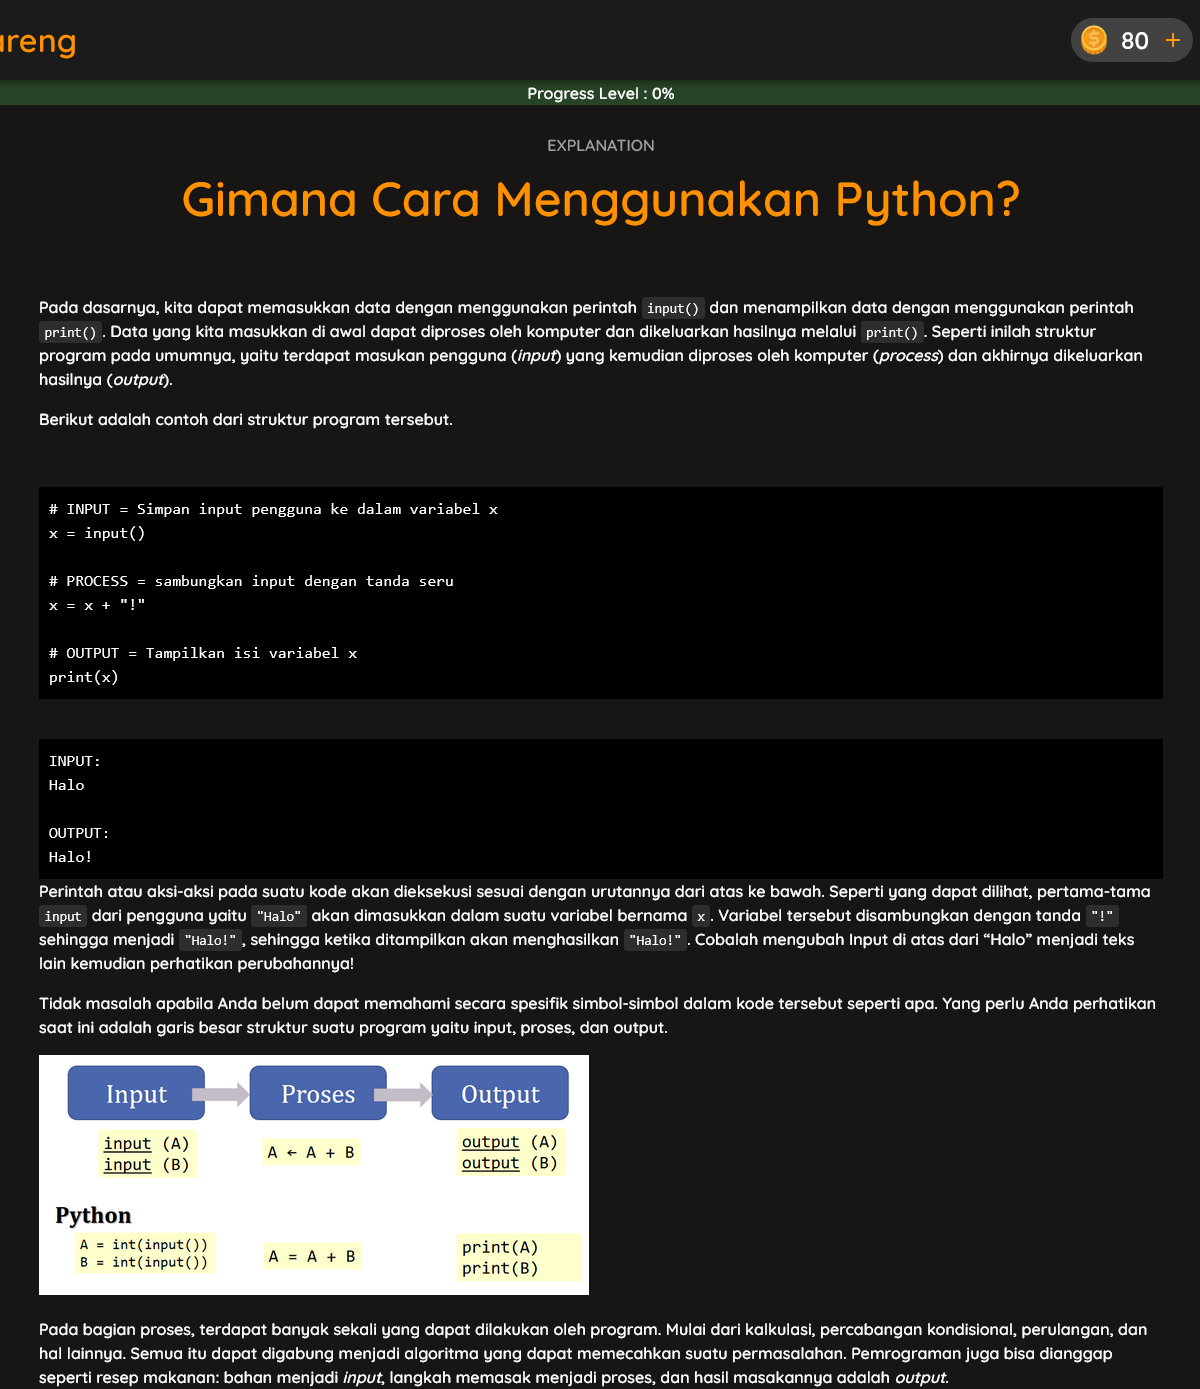
\includegraphics[width=0.7\textwidth]{chapter2/kodebareng-materi.png}
  \caption{Materi pembelajaran Python Dasar di Kodebareng \\ Sumber: Penulis (2022)}\label{fig:kodebareng-materi}
\end{figure}

Latihan soal pada KodeBareng memiliki 2 jenis soal, yaitu soal kuis dan soal latihan kode. Soal kuis merupakan soal yang berupa pilihan ganda dengan jawaban yang selalu diacak urutannya, serta hanya memiliki 1 jawaban yang benar (seperti pada \autoref{fig:kodebareng-soal-kuis}). Apabila salah menjawab, pelajar akan diberitahu dengan \textit{pop-up dialog} "Jawaban Salah" lalu dapat mencoba menjawab kembali dengan jawaban yang lain. Soal latihan kode merupakan soal yang berupa permasalahan yang diberikan secara teks, lalu pelajar diminta untuk membuat atau mengubah kode yang sudah ada untuk menyelesaikan permasalahan tersebut dengan cara mengecek jawabannya pada \textit{autograder} yang telah disediakan (tampilan dapat dilihat pada \autoref{fig:kodebareng-soal-latihankode}). Apabila jawabannya salah, maka pelajar tidak dapat melanjutkan pembelajaran hingga jawaban yang benar ditemukan.

\begin{figure}[H]
  \centering
  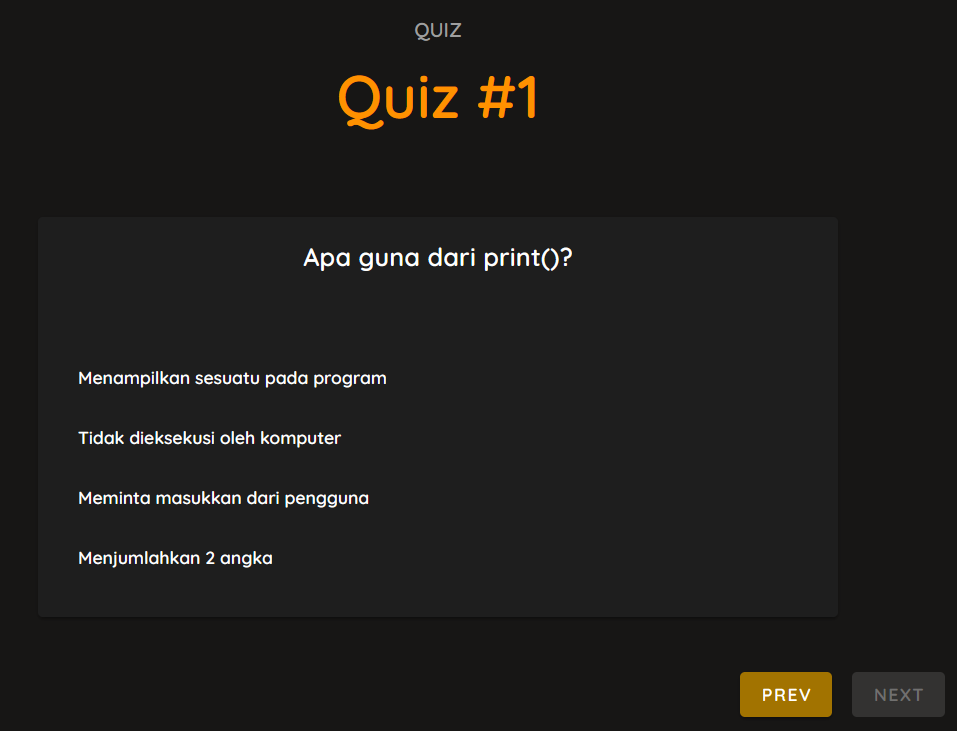
\includegraphics[width=0.55\textwidth]{chapter2/kodebareng-soal-kuis.png}
  \caption{Contoh soal kuis Python Dasar di Kodebareng \\ Sumber: Penulis (2022)}\label{fig:kodebareng-soal-kuis}
\end{figure}

\begin{figure}[H]
  \centering
  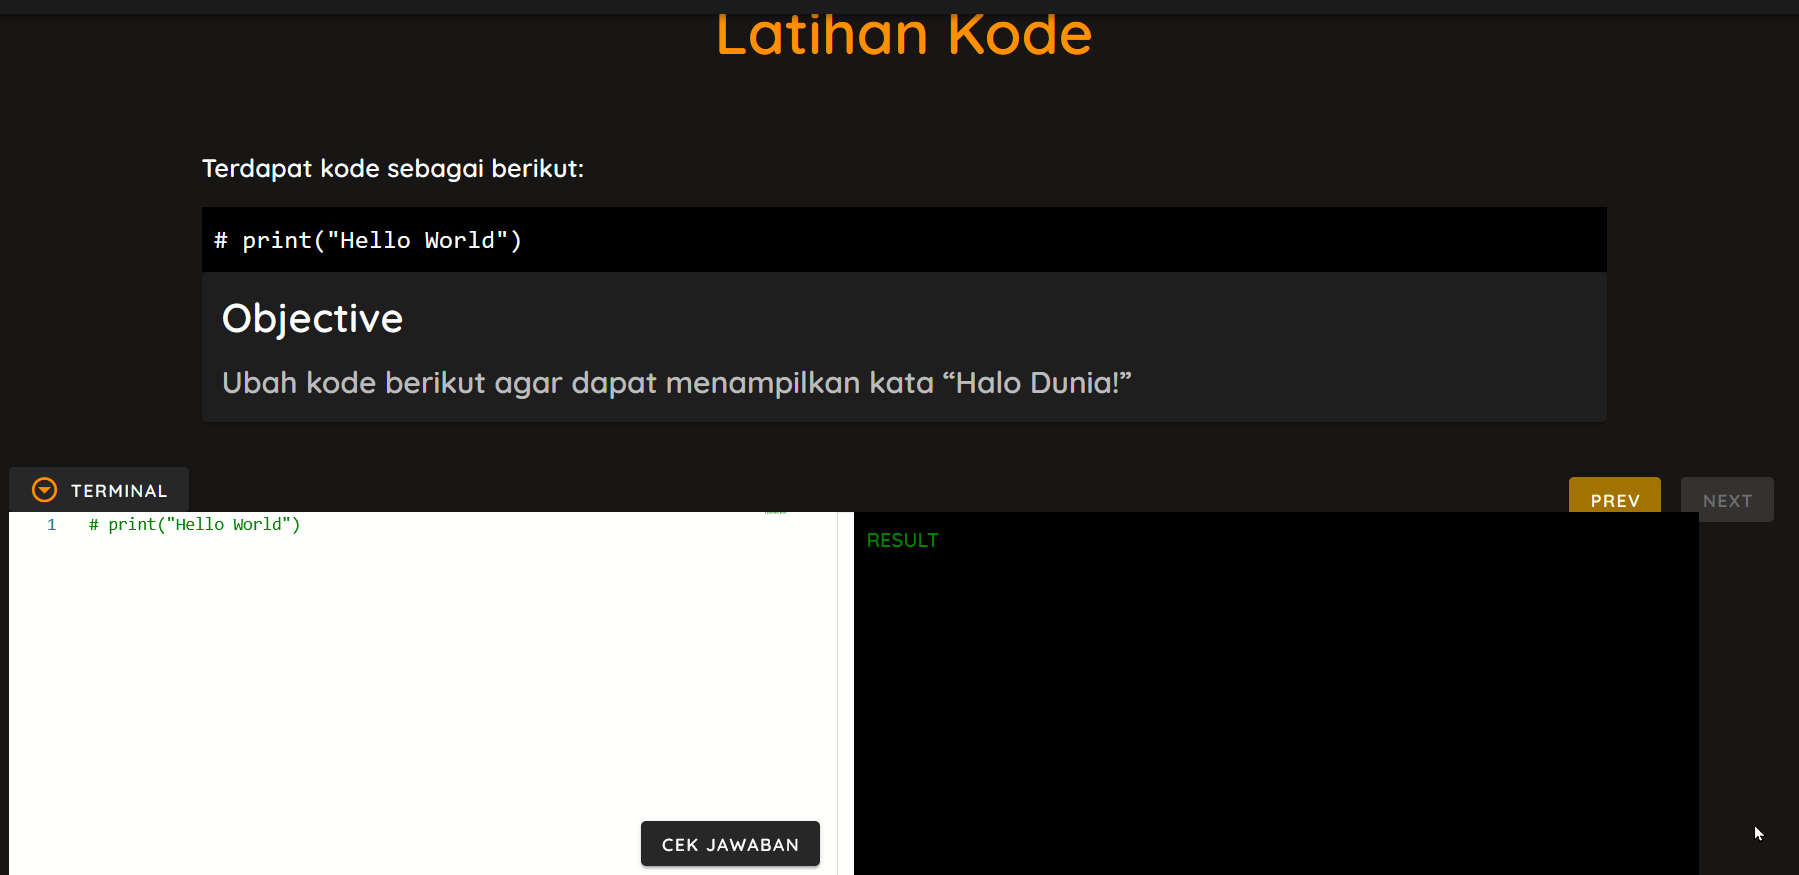
\includegraphics[width=0.8\textwidth]{chapter2/kodebareng-soal-latihankode.png}
  \caption{Contoh soal latihan kode Python Dasar di Kodebareng \\ Sumber: Penulis (2022)}\label{fig:kodebareng-soal-latihankode}
\end{figure}

Karena pembelajaran interaktif pada KodeBareng masih hanya sebatas pembawaan materi, pengalaman pembelajarannya masih dianggap kurang interaktif dan sama dengan platform kelas pembelajaran pemrograman lainnya seperti yang telah dibahas pada \autoref{sssec:ragam-implementasi-ile}. Maka dari itu, dibutuhkan suatu \textit{interactive learning environment} (ILE) yang dapat mendukung pembelajaran interaktif dan memecahkan masalah sulitnya mempelajari pemrograman bagi orang yang baru mempelajari pemrograman. ILE diharapkan dapat meningkatkan pemahaman konsep serta mendukung pemrograman praktis pelajar. ILE dibangun secara modular pada platform KodeBareng sehingga tidak terlalu disruptif terhadap sistem yang sudah ada. Berikut adalah diagram \textit{use case} awal KodeBareng yang terkait dengan pembelajaran pemrograman yang dapat dilihat pada \autoref{fig:diagram-usecase-v1}.

\begin{figure}[H]
  \centering
  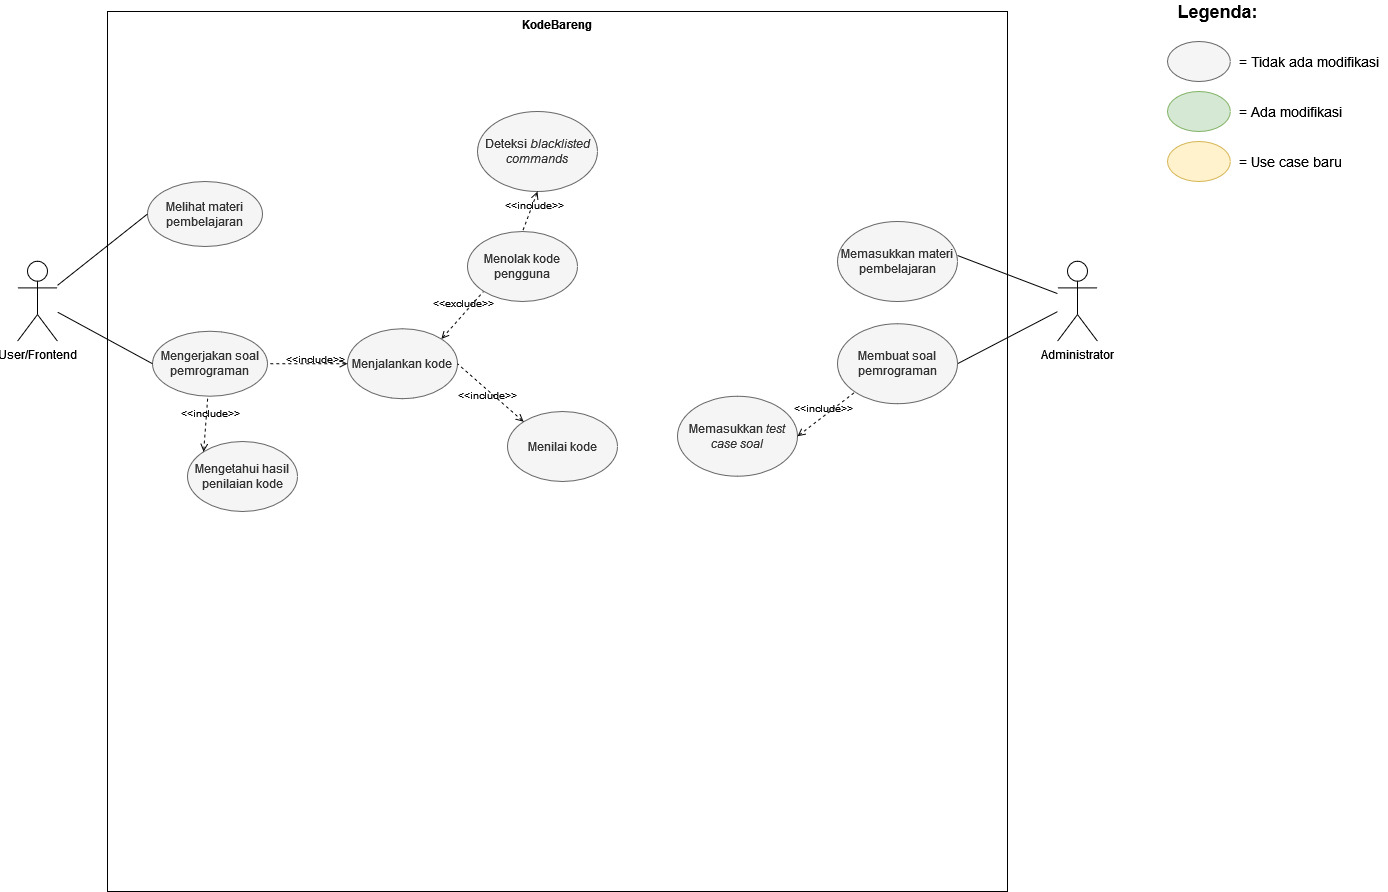
\includegraphics[width=0.9\textwidth]{chapter3/diagram_usecase_v1.jpg}
  \caption{\textit{Use Case} pembelajaran pemrograman KodeBareng sebelum perubahan \\ Sumber: Penulis (2022)} \label{fig:diagram-usecase-v1}
\end{figure}